\documentclass[a4paper]{article}


\usepackage{fullpage}               % Reduce white space around margins
\usepackage{graphicx}               % For including images
\usepackage{chngcntr}               % For section-wise table/figure counters
\usepackage{caption}                % For specifying figure/table captions and its attributes
\usepackage{geometry}               % For specifying margin sizes
\usepackage{amssymb}                % For simple math symbols
\usepackage{verbatimbox}            % For a neat box around verbatim text
\usepackage{multirow,tabularx}      % For row splits in a table
\usepackage{fancyvrb}               % For super/sub script text within verbatim block
\usepackage{fixltx2e}               % For super/sub script text within verbatim block


\date{}                             % Don't print the date
\linespread{1.5}                    % Line spacing = 1.5
\counterwithin{table}{section}      % Count tables per-section
\counterwithin{figure}{section}     % Count figures per-section
\geometry{a4paper, margin=0.82in}


\begin{document}


% Create title page
    \begin{titlepage}
        \vspace*{\fill}
        \begin{center}
            {\huge \bf ECE 521 - Computer Design Techniques \\ Fall 2014 \\ \vspace {8 mm} \\ \LARGE \bf Branch Predictor Implementation \\ \vspace{4 mm} Project Report}
            
            {\vspace{9 mm} \it \large Prepared by \\ \bf \Large Aravindhan Dhanasekaran\\ \bf \large adhanas@ncsu.edu}
        \end{center}
        \vspace*{\fill}
    \end{titlepage}


\pagenumbering{roman}
\newpage
\tableofcontents
\listoffigures
\listoftables
\newpage
\pagenumbering{arabic}


\section{Introduction}
In this project, a branch predictor has been built which can simulate 3 types of branch predictors: bimodal, gshare and hybrid. Also, set-associative Branch Target Buffer (BTB) cache support is available, using which a branch can be predicted during instruction fetch cycle itself. The BTB uses LRU replacement policy to age out entries.

\section{Formulas}
Some of the important formulas that are used to characterize branch predictor performance are briefly discussed in this section.

\subsection{Program Counter to Branch Predictor Table Index Conversion}
The branch instruction addresses are always 4-byte aligned starting from 0. Thus, the last two bits of all addresses will be zero. Since, we use a part of lower order bits of the instruction address as an index to the predictor table, we need to ignore the leftmost 2-bits to minimize collisions.

\subsubsection{Index Calculation for Bimodal Predictor}
The bimodal predictor table index for bimodal predictor can be calculated using the below formula.

\begin{verbatim}
                            pc >>= 2;
                            index = m-bit lower order mask
                            index &= pc
\end{verbatim}

\subsubsection{Index Calculation for Gshare Predictor}
In gshare preditor, the global history register is also used in index calculation. This minimizes the number of collisions in the predictor table. The gshare predictor table index for bimodal predictor can be calculated using the below formula.

\begin{verbatim}
                            pc >> = 2
                            index = m-bit lower order mask
                            index &= pc
                            index ^= bhr
\end{verbatim}

\subsubsection{Index Calculation for Hybrid Predictor}
The hybrid predictor uses a 2\textsuperscript{k} bit chooser table for prediction. Its index is calculated similar to bimodal index.

\begin{verbatim}
                            pc >>= 2;
                            index = k-bit lower order mask
                            index &= pc
\end{verbatim}

\subsection{Misprediciton Rate}
Misprediciton rate denotes the ratio of number of branch mispredicitons (predicted differently from the actual branch outcome) by the predictor to the total number of branches. The lower the misprediction rate, the better is the perdictor's performance. This rate is one of the important attribute of a predictor which helps in understanding the characteristics it. All predictor performance improvement  methods would decrease the misprediction rate in one way or the other.

\[mispredicitonRate = \frac{numMisPredicitons}{numTotalBranches}\]

\subsection{Predictor Table Size}
The predictor table size is determined by the number of bits that are available to index the table (i.e,2\textsuperscript{num of bits in index}), which is in turn governed by the value 'm'. 

\begin{Verbatim}[commandchars=\\\{\},codes={\catcode`$=3\catcode`_=8}]
            Size of predictor table = (# of bits in counter) * (2\textsuperscript{m}) bits
\end{Verbatim}

\section{Experiments}
Various experiments with bimodal and gshare predictors were run in order to understand the predictor's performance affecting attributes. This section represents the different runs, predictor parameters and statistics of every run in tables and in graphs. The data will be analyzed in following section.

In all the following experiments, three different trace files are used: gcc\_trace, jpeg\_trrace and perl\_trace.

\subsection{Bimodal Predictor Experiments}
In this experiment, the 2-bit bimodal predictor is tested against different values of m (the number of lower order bits of PC to be used as an index of the predictor table) and different benchmarks - gcc, jpeg and perl. The misprediction rate is calculated in each case and plotted against the m value. This data is available in table \ref{tab:bimodal} and the reuslts are plotted as graphs in figures \ref{fig:bimodal_gcc}, \ref{fig:bimodal_jpeg} and \ref{fig:bimodal_perl}. 

\begin{figure} [htbp]
    \centering
    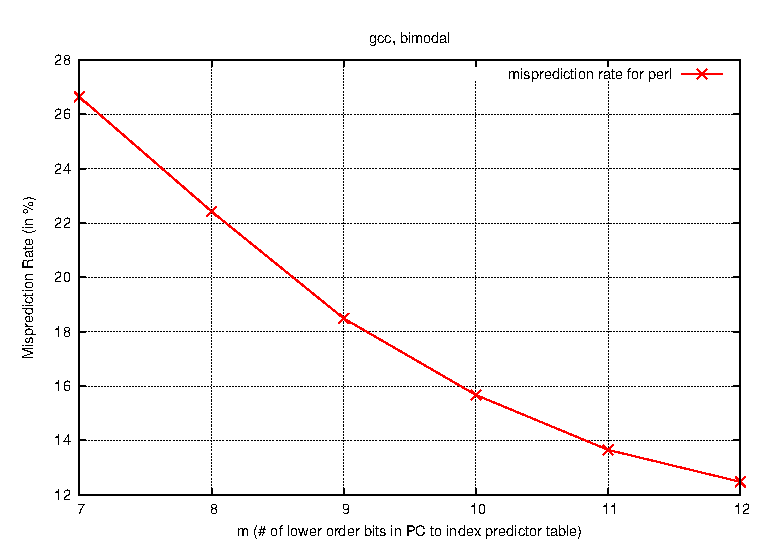
\includegraphics[scale=1.32] {image/gcc_bimodal.eps}
    \caption{Bimodal predictor misprediction rate for gcc trace}
    \label{fig:bimodal_gcc}
\end{figure}

\begin{table}[htbp]
    \centering
    \begin{tabular}{|c|c|c|c|}
        \hline
        \multirow{2}[3]{*}{\bf m (bits) } & \multicolumn{3}{c|}{\bf Misprediction Rate} \\
        \cline{2-4} & \bf gcc & \bf jpeg & \bf perl \\
        \hline
             7 & 26.65 & 7.92 & 21.31 \\
             8 & 22.43 & 7.79 & 16.45 \\
             9 & 18.49 & 7.74 & 14.14 \\
            10 & 15.67 & 7.70 & 11.95 \\
            11 & 13.65 & 7.62 & 11.05 \\
            12 & 12.47 & 7.60 &  9.09 \\
            13 & 11.72 & 7.59 &  8.92 \\
            14 & 11.37 & 7.59 &  8.82 \\
            15 & 11.30 & 7.59 &  8.82 \\
            16 & 11.21 & 7.59 &  8.82 \\
        \hline
    \end{tabular}
    \captionsetup{justification=centering}
    \caption{Experiment Data for bimodal predictor for different `m' values and traces}
    \label{tab:bimodal}
\end{table}

\begin{figure} [htbp]
    \centering
    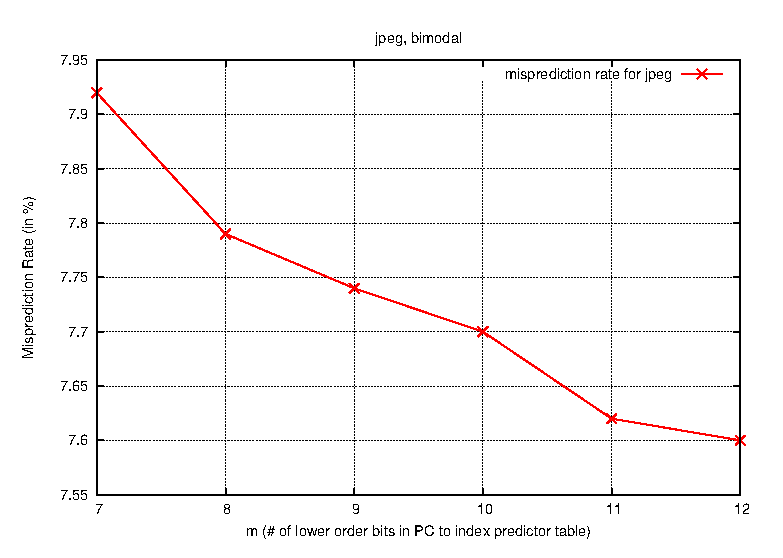
\includegraphics[scale=1.32] {image/jpeg_bimodal.eps}
    \caption{Bimodal predictor misprediction rate for jpeg trace}
    \label{fig:bimodal_jpeg}
\end{figure}

\begin{figure} [htbp]
    \centering
    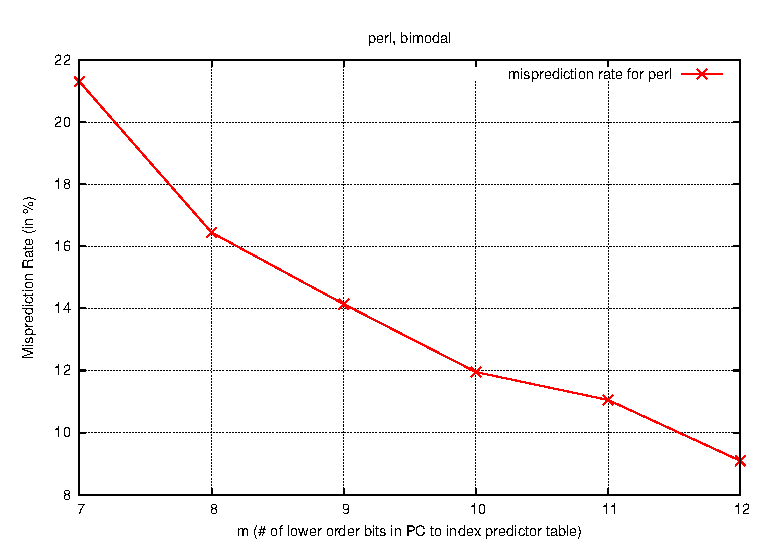
\includegraphics[scale=1.32] {image/perl_bimodal.eps}
    \caption{Bimodal predictor misprediction rate for perl trace}
    \label{fig:bimodal_perl}
\end{figure}

\subsection{Gshare Predictor Experiments}
In this experiment, the ghsare branch predictor is run against different values of m (the number of lower order bits of PC to be used as an index of the predictor table), n (the number of bits in global branch history register) and different benchmarks - gcc, jepg and perl. The misprediction rate is calculated in each case and plotted against the m value. This data is available in tables \ref{tab:gshare_gcc}, \ref{tab:gshare_jpeg} and \ref{tab:gshare_perl} and the results are plotted as graphs in figures \ref{fig:gshare_gcc}, \ref{fig:gshare_jpeg} and \ref{fig:gshare_perl}.

\begin{table}[htbp]
    \centering
    \begin{tabular}{|c|c|c|c|c|c|c|}
        \hline
        \multirow{2}[6]{*}{\bf m (bits) } & \multicolumn{6}{c|}{\bf Misprediction Rate} \\
        \cline{2-7} & \bf n = 2 & \bf n = 4 & n = 6 & \bf n = 8 & \bf n = 10 & \bf n = 12 \\
        \hline
         7 & 28.98 & 30.76 & 32.22 & - & - & - \\
         8 & 25.81 & 26.57 & 27.82 & 30.56 & - & - \\
         9 & 20.25 & 22.43 & 24.14 & 26.08 & - & - \\
        10 & 16.39 & 17.99 & 19.36 & 21.10 & 22.77 & - \\
        11 & 13.71 & 14.49 & 15.14 & 16.47 & 18.34 & - \\
        12 & 12.20 & 12.23 & 12.46 & 13.00 & 14.33 & 15.40 \\
        \hline
    \end{tabular}
    \captionsetup{justification=centering}
    \caption{Experiment Data for gshare predictor for different `m' and `n' values for gcc trace}
    \label{tab:gshare_gcc}
\end{table}

\begin{figure} [htbp]
    \centering
    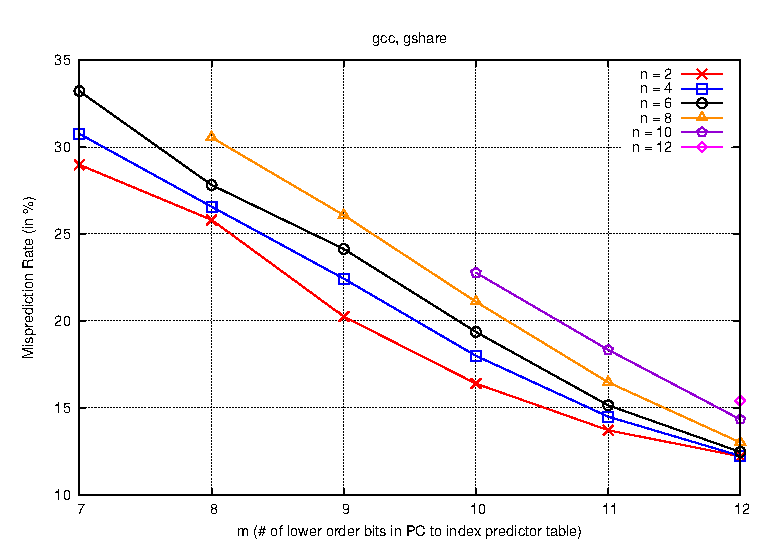
\includegraphics[scale=1.32] {image/gcc_gshare.eps}
    \caption{Ghsare predictor misprediction rate for gcc trace}
    \label{fig:gshare_gcc}
\end{figure}

\begin{table}[htbp]
    \centering
    \begin{tabular}{|c|c|c|c|c|c|c|}
        \hline
        \multirow{2}[6]{*}{\bf m (bits) } & \multicolumn{6}{c|}{\bf Misprediction Rate} \\
        \cline{2-7} & \bf n = 2 & \bf n = 4 & n = 6 & \bf n = 8 & \bf n = 10 & \bf n = 12 \\
        \hline
         7 & 8.08 & 8.92 & 9.74 & - & - & - \\
         8 & 7.79 & 7.88 & 8.87 & 9.20 & - & - \\
         9 & 7.58 & 7.68 & 8.13 & 8.30 & - & - \\
        10 & 7.49 & 7.38 & 7.58 & 7.45 & 7.95 & - \\
        11 & 7.45 & 7.27 & 7.38 & 7.17 & 7.44 & - \\
        12 & 7.44 & 7.26 & 7.19 & 6.84 & 7.18 & 7.35 \\
        \hline
    \end{tabular}
    \captionsetup{justification=centering}
    \caption{Experiment Data for gshare predictor for different `m' and `n' values for jpeg trace}
    \label{tab:gshare_jpeg}
\end{table}

\begin{figure} [htbp]
    \centering
    \includegraphics [scale=1.32] {image/jpeg_gshare.eps}
    \caption{Gshare predictor misprediction rate for jpeg trace}
    \label{fig:gshare_jpeg}
\end{figure}

\begin{table}[htbp]
    \centering
    \begin{tabular}{|c|c|c|c|c|c|c|}
        \hline
        \multirow{2}[6]{*}{\bf m (bits) } & \multicolumn{6}{c|}{\bf Misprediction Rate} \\
        \cline{2-7} & \bf n = 2 & \bf n = 4 & n = 6 & \bf n = 8 & \bf n = 10 & \bf n = 12 \\
        \hline
         7 & 24.34 & 25.96 & 28.71 &     - &     - &    - \\
         8 & 16.92 & 19.09 & 20.45 & 24.79 &     - &    - \\
         9 & 13.57 & 14.68 & 16.25 & 17.66 &     - &    - \\
        10 & 10.63 & 11.35 & 11.52 & 12.42 & 14.57 &    - \\
        11 & 10.11 &  9.68 &  8.60 &  9.00 &  8.98 &    - \\
        12 &  9.04 &  8.09 &  7.50 &  6.49 &  6.71 & 7.16 \\
        \hline
    \end{tabular}
    \captionsetup{justification=centering}
    \caption{Experiment Data for gshare predictor for different `m' and `n' values for perl trace}
    \label{tab:gshare_perl}
\end{table}

\begin{figure} [htbp]
    \centering
    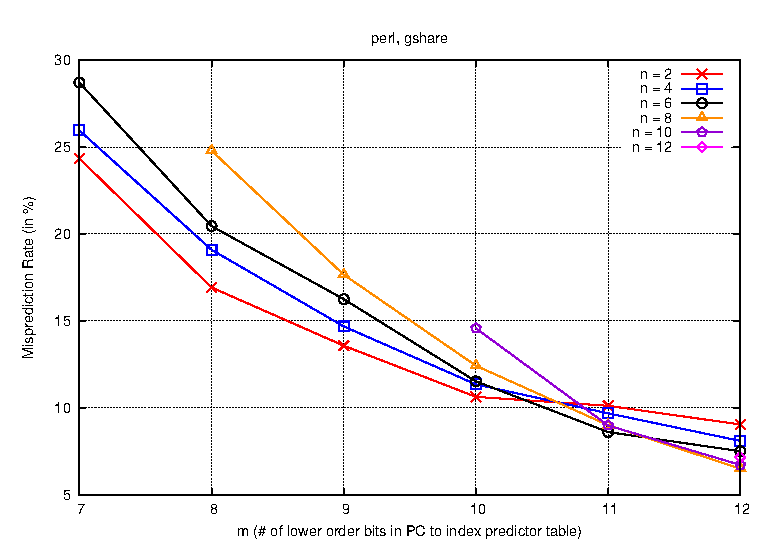
\includegraphics [scale=1.32] {image/perl_gshare.eps}
    \caption{Gshare predictor misprediction rate for perl trace}
    \label{fig:gshare_perl}
\end{figure}


\section{Branch Predictor Performance Analysis}
The branch predictor's performance depends on many factors such as number of bits available to store the history of predictions, size of the predictor table, size of the branch target buffer and the branch instruction patterns themselves. In this section, we will analyze the data that we obtained in section 3 for bimodal and ghsare predictors.

\subsection{Analysis of Bimodal Predictor}
From the graphs in figures \ref{fig:bimodal_gcc}, \ref{fig:bimodal_jpeg} and \ref{fig:bimodal_perl}, it can be clearly seen that the misprediction rate decreases as `m' value increases. This is due to the fact that using more bits of PC to index the predictor table reduces the collision domain of branch instructions in the predictor table. But, this also increases the storage cost as every additional bit used doubles the memory requirements. 

\subsubsection{Benchmark Comparison}
From table \ref{tab:bimodal} it can be inferred that jpeg trace has the lowest misprediction rate among all given benchmarks, followed by perl and finally gcc. This could be attributed to the reason that jpeg benchmark has the branch instructions in a widely distributed manner thus reducing the collisions within the predictor table.

\subsubsection{Best Design Selection}
In this section, we choose the best possible design (lowest misprediction rate) for each given benchmark with the constraint that the size of the predictor table should be no more than 16 KB.

From section 2.3, we know that the size of the bimodal predictor table is defined by `m'. i.e., size of the predictor table = 2 * 2\textsuperscript{m} bits.

\begin{itemize}
\item gcc: For a bimodal predictor table size of 16KB, we can use up to 16 bits in PC (2 * 2\textsuperscript{17}/8192 = 16 KB). From table \ref{tab:bimodal}, it can be observed that for m = 16 and gcc trace, the misprediction rate is 11.21, which is better than the rates for lower values of m.

\item jpeg: For jpeg trace in table \ref{tab:bimodal}, bimodal predictor misprediction rate saturates at m = 13. So, we can build a table of size (2 * 2\textsuperscript{13}) = 2 KB.

\item perl: For m = 13, the misprediction rate is 8.92 and for higher values of m, the misprediction rate is less by a negligible value. So, we can safely build a predictor table of size 2 KB.
\end{itemize}

\subsection{Analysis of Gshare Predictor}
From the graphs in figures \ref{fig:gshare_gcc}, \ref{fig:gshare_jpeg} and \ref{fig:gshare_perl} it can be inferred that the misprediciton rate decreases as `m' increases as expected. The curve flattens for higher values of `m' (for gcc) and for higher values of `n' (for jpeg and perl).

But, the graphs also exhibit ``laws of dimnishing" returns for `n' value. i.e,, while increasing `n' enables more bits in history register to XOR with PC (thus minimizing the collision domain), it increases the overall misprediction rate of the predictor. 

\subsubsection{Benchmark Comparison}
The benchmarks for ghsare are similar to that of bimodal predictor. The jpeg trace has much more wide distribution of the branch instructions in the predictor tables (and thus has less collisions) and thereby has the lowest misprediction rate. Of the remaining two, perl has better misprediction rate than gcc trace. The results of the experiments for different benchmarks are tabulated in tables \ref{tab:gshare_gcc},\ref{tab:gshare_jpeg} and \ref{tab:gshare_perl} for reference. 

\subsubsection{Best Design Selection}
In this section, we choose the best possible design (lowest misprediction rate) for each given benchmark with the constraint that the size of the predictor table should be no more than 16 KB.

From section 2.3, we know that the size of the predictor table is defined by `m'. i.e., size of the predictor table = 2 * 2\textsuperscript{m} bits.

\begin{itemize}
\item gcc: From table \ref{tab:gshare_gcc}, it can be seen that the misprediction rate is lower for lower values of n. i.e., for m \textless 14 and n = 2, the misprediciton rate is less. Also, the misprediction rate is less by a negligible value for m \textgreater 13. So, we can use m = 13 and n = 2 for our predictor table to get best results. The size of the predictor table for this configuration will be ((2\textsuperscript{13}/8) * 2) = 2 KB, \textless 16 KB constraint.

\item jpeg: From the graph in figure \ref{fig:gshare_jpeg}, it is very clear that the misprediction rate is the lowest for n = 8 and m = 12. The size of the predictor table for such a configuration would be ((2\textsuperscript{12}/8) * 2) = 1 KB, which is way less than the 16 KB constraint.

\item perl: Similar to jpeg benchmark, the misprediction rate is lowest for n = 8 and m = 12 for perl benchmark from table \ref{tab:gshare_perl}. The curve in figure \ref{fig:gshare_perl} flattens out for higher values of n and m after that. So, the predictor table size would be similar to that of jpeg benchmark, 1 KB.
\end{itemize}


\section{Conclusion}
The key takeaway of this project and the project report is the understanding of different branch predictors and their attributes and how it affects the performance of a predictor (in both positive and negative way). The experiments and the associated plots shows that the `m' value of a predictor plays an important role in bringing down the misprediction rate. Other factors include `n' value and branch target buffer size.


\end{document}
